%%% Lecture 5

\lecture[A lot of simplicial stuff.]{2021-10-27}

Given two simplicial sets $X$ and $Y$, their product $X\times Y$ is the functor \[\Delta^\op\xto{(X,Y)}\Set\times\Set\xto{\times}\Set\] i.e. $(X\times Y)_n=X_n\times Y_n$ and $\alpha^*_{X\times Y}=\alpha^*_X\times\alpha^*_Y$.

The \textbf{simplicial $n$-simplex} is the represented simplicial set $\Delta[n]:=\Delta(-,[n])$. By the Yoneda lemma, for every simplicial set $X$, the map $\sSet(\Delta[n],X)\to X_n$, $(f:\Delta[n]\to X)\mapsto f_n(\id_{[n]})$.

A \textbf{homotopy between morphisms} $f,g:X\to Y$ in $\sSet$ is a morphism $H:X\times\Delta[1]\to Y$ such that $H\circ i_0=f$ and $H\circ i_1=g$, where $i_0,i_1:X\to X\times\Delta[1]$ (note: the morphism $i_0$ has components $(i_0)_n:X_n\to X_n\times\Delta([n],[1])$, $x\mapsto(x,\text{cost}_0)$).

The topological simplex $\nabla^n=\cb{(\xso)\in\R^{n+1}\mid x_i\geq0,\ \sum x_i=1}$ has a preferred CW-structure with $\sk_k(\nabla^n)=\cb{(\xso)\in\nabla^n\mid\text{at most }k+1\text{ cordinates are non-zero}}$, i.e. $\sk_k(\ns)$ is the union of all $k$-dimensional faces of $\ns$:
\begin{itemize}
    \item $\sk_0(\nabla^n)=\cb{\nno{e}{n}}$,
    \item $\sk_j=\dots$
    \item $\sk_{n-1}(\nabla^n)=\de\nabla^n$,
    \item $\sk_n(\nabla^n)=\nabla^n$.
\end{itemize}\medskip

Let $(X,A)$ be a space pair and $k\geq-1$. We define a \textbf{simplicial subset} $\S(X,A,k)$ of $\S(X)$ by setting
\[S(X,A,k)_n=\cb{f:\ns\to X\mid f(\sk_k(\ns))\subset A}.\]
This is indeed a simplicial subset because the affine linear maps $\alpha_*:\ns\to\ms$ are cellular.

Note that we have:

\[\S(X)=\S(X,A,-1)\supset \S(X,A,0)\supset \S(X,A,1)\supset\dots\supset\bigcap_{k\geq1}\S(X,A,k)=\S(A).\]

A space pair $(X,A)$ is \textbf{$k$-connected}, $h\geq0$, if the following equivalent conditions hold:
\begin{enumerate}[label={(\alph*)},topsep=0.5\thmsep]
    \item The inclusion $A\hto X$ is a bijection on $\pi_i$ for all $i<k$ and all basepoints in $A$ and a surjection on $\pi_k$,
    \item Every pair map $(D^n,\de D^n)\to (X,A)$ for $0\leq n\leq k$ is homotopic relative $\de D^n$ to a map with image in $A$,
    \item The map $\pi_0(A)\to \pi_0(X)$ is surjective and $\pi_i(X,A,x)=\cb{*}$ for all $1\leq i\leq k$ and all $x\in A$.
\end{enumerate}

We want to prove the following theorem.

\begin{theorem**}
Let $(X,A)$ be a $k$-connected pair of spaces. The inclusion $\S(X,A,k)\hto\S(X)$ is then a deformation retraction of simplicial sets.
\end{theorem**}

This means there is a simplicial homotopy
\[H:S(X)\times\Delta[1]\to S(X)\]
from the identity to a morphism with image in $\S(X,A,k)$ that is relative to $\S(X,A,k)$, i.e. the restriction of $H$ to $S(X,A,k)$ is the composite
\[\S(X,A,k)\times\Delta[1]\xto{\text{proj}}\S(X,A,k)\xhto{\text{incl}}\S(X).\]

We first prove a proposition.

Let $X$ be a simplicial set and $x\in X_n$, for $n\geq0$. Then the $n$-simplex $x$ is \textbf{degenerate} if there is a surjective morphism $\sigma:[n]\to [k]$ with $k<n$, and $y\in X_k$ such that $X=\sigma^*(y)$ (i.e. $x\in\im(\sigma^*:X_k\to X_n)$).

\begin{proposition}
Let $X$ be a simplicial set and $x\in X_n$. Then there is a unique pair $(\sigma,y)$ consisting of:
\begin{itemize}
    \item a surjective morphism $\sigma: [n]\to [k]$ and
    \item a non-degenerate simplex $y\in X_k$
\end{itemize}
such that $X=\sigma^*(y)$.
\end{proposition}

\begin{proof}\ 

Existence. By induction on $n$. If $n=0$ then $X$ is non-degenerate and $(\id_{[0]},x)$ does the job.

For $n\geq1$: if $x$ is non-degenerate, then $(\id_{[n]},x)$ does the job.
Otherwise $x=\sigma^*(x')$ for some $\sigma:[n]\to [k]$, $k<n$, $x'\in X_k$.
Then $x'=(\sigma')^*(y)$ for some surjective morphism $\sigma':[k]\to[l]$ and $y\in X_l$ non-degenerate, by induction. Then \[x=\sigma^*(x')=\sigma^*((\sigma')^*(y))=(\sigma'\circ\sigma)^*(y)\] which is the desired expression.

Uniqueness. Let $x=\sigma^*(y)=\bar{\sigma}^*(\bar y)$ for surjective morphisms $\sigma:[n]\onto[k]$, $\bar{\sigma}:[n]\onto[l]$ and $y\in X_k$, $\bar y \in X_l$ non-degenerate.

Let $\delta:[k]\to[n]$ be a morphism in $\Delta$ such that $\sigma\circ\delta=\id_{[k]}$.
Then
\[y=(\sigma\delta)^*(y)=\delta^*(\sigma^*(y))=\delta^*(\bar{\sigma}^*(\bar{y}))=(\bar{\sigma}\delta)^*(\bar{y})\]
We write
\[\bar{\sigma}\delta=\delta'\sigma': [k]\to[l]\]
where $\sigma':[k]\onto[a]$ is surjective and $\delta':[a]\hto[l]$ is injective. Then \[y=(\bar\sigma\delta)(\bar y)=(\delta'\sigma')^*(\bar y)=(\sigma')^*((\delta')^*(\bar{y}))\tag{$*$}\]

Since $y$ is non-degenerate, we must have $a=k$ and $\sigma'=\id_{[k]}$. Hence $k=a\leq l$. By interchanging the roles of $(\sigma,y)$ and $(\bar{\sigma},\bar{y})$ we obtain $l\leq k$, hence $l=k$.

Then by $(*)$ we have $y=(\delta')^*(\bar{y})$ so $\delta'=\id$ and hence $y=\bar{y}$ and $\sigma=\bar{\sigma}$.
\end{proof}

\begin{theorem}\label{sx-def-r}
Let $(X,A)$ be $k$-connected. Then $S(X,A,k)\hookrightarrow S(X)$ is a simplicial deformation retraction.
\end{theorem}

\begin{proof}
We will construct the following data. Continuous maps $\psi_f:\nabla^n\times\nabla^1\to X$ for all $f:\nabla^n\to X$, $n\geq 0$, such that:
\begin{enumerate}[label={(\alph*)}]
    \item $\psi_f(-,e_0)=f$, $\psi_f(\sk_k(\ns),e_1)\subset A$.
    \item If $f(\sk_k(\ns))\subset A$, then $\psi_f=f\circ\pr_1$.
    \item The maps $\psi_f$ are compatible in the simplicial direction, i.e. for all $\alpha:[n]\to[m]$, $g:\nabla^m\to X$, the following commutes:
    \begin{center}
        \begin{tikzcd}
            \nabla^n\times\nabla^1 \arrow[d, swap, "\alpha_*\times\id"] \arrow[r, "\psi_{\alpha^*(g)}"] & X \\
            \nabla^m\times\nabla^1 \arrow[ur, swap, "\psi_g"]
        \end{tikzcd}
    \end{center}
\end{enumerate}

Construction of the $\psi_f$'s. By induction on $n\geq0$.

$(n=0)$ The map $f:\nabla^0\to X$ is determined by its image $f(e_0)\in X$. Since $\pi_0(A)\to\pi_0(X)$ is surjective, we can choose a path from $f(e_0)$ to some point in $A$. We view the path as a continuous map $\psi_f:\nabla^0\times\nabla^1\to X$ with $\psi_f(e_0,e_0)=f(e_0)$, $\psi_f(e_0,e_1)\in A$. If $f(e_0)\in A$, we take the constant path at $f(e_0)$.

$(n\geq1)$ We distinguish three cases:

Case 1. $f:\nabla^n\to X_n$ is degenerate as a simplex of the simplicial set $\S(X)$. Then $f=\sigma^*(g)$ for a unique pair $(\sigma,g)$ with $\sigma:[n]\onto[k]$, $k<n$ and $g:\nabla^k\to X$ continuous. By (c) we have to define $\psi_f$ as the composite
\[\nabla^n\times\nabla^1\xto{\sigma_*\times\id}\nabla^k\times\nabla^1\xto{\psi_g} X\]

Case 2. $f:\nabla^n\to X$ is non-degenerate and $k<n$. We note that by property $(c)$, the map $\psi_f:\nabla^n\times\nabla^1\to X$ is already fixed on $(\de\nabla^n)\times\nabla^1$; by $(a)$ it is also determined on $\nabla^n\times e_0$.

We extend the data to $\nabla^n\times\nabla^1$ by a choice of continuous retraction:
\[r:\nabla^n\times\nabla^1\to (\nabla^n\times e_0)\cup(\de\nabla^n\times\nabla^1)\]
hence set $\psi_f$ to be the composite of $r$ and $\til f=f\cup\bigcup_{i=0,\dots,n}\psi_{d_i^*(f)}$\normalmarginpar\marginnote{\footnotesize $d_i:[n-1]\to[n]$ is the unique monotone injection with $i\not\in\im(d_i)$).}:
\[\ns\times\sx{1}\xto{r}(\nabla^n\times e_0)\cup(\de\nabla^n\times\nabla^1)\xto{\til f} X\]

The definition satisfies $\psi_f(-,e_0)=f$ by design and $\psi_f(\sk_k(\nabla^n),e_1)\subset\psi_f(\de\nabla^n,e_1)\subset A$ by induction because $\psi_{d_i^*(f)}$ have property $(a)$.

Case 3. $f:\nabla^n\to X$ is non-degenerate and $n\leq k$. First, note that we can show the pair $((\nabla^n\times e_0)\cup(\de\nabla^n\times\nabla^1), \de\nabla^n\times e_1)$ to be pair homeomorphic to $(D^n,\de D^n)$.

We assumed that $(X,A)$ is $k$-connected, so there are a continuous map $\lambda$ and a homotopy from $\lambda$ to the map $\til f=f\cup\bigcup_{i=0,\dots,n} \psi_{d_i^*(f)}$

\[\lambda:(\nabla^n\times e_0)\cup(\de\nabla^n\times\nabla^1)\to A\]
\[H:(\nabla^n\times e_0)\cup(\de\nabla^n\times\nabla^1)\times[0,1]\to X\]

which combine in the diagram (where the lower triangle is commutative up to homotopy):
\begin{center}
    \begin{tikzcd}[column sep=huge]
    (\de\ns\times e_1) \arrow[r, "\bigcup_{i=0,\dots,n} \psi_{d_i^*(f)}"] \arrow[d, hook] & A \arrow[d, hook] \\
    (\ns\times e_0)\cup(\de\ns\times\sx{1}) \arrow[ur, dashed, swap, "\lambda"] \arrow[r, swap, "\til f"] & X
    \end{tikzcd}
\end{center}

\[\begin{tikzcd}
	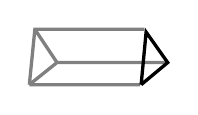
\begin{tikzpicture}[x=2em, y=2em]
    \draw[very thick, black!50]
        (0,0)--(2,0)
        (2.075,1)--(0.1,1)--(0,0)
        (0,0)--(0.5,0.4)--(0.1,1)
        (0.5,0.4)--(2.5,0.4);
	\draw[very thick] (2.02,0)--(2.5,0.4)--(2.11,0.95)--(2.02,0);
    \end{tikzpicture}
	 && A \\
	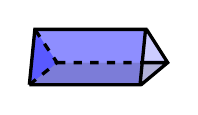
\begin{tikzpicture}[x=2em, y=2em,baseline=0.5em]
    \begin{scope}[very thick]
    \fill[fill=blue, opacity=0.3]
        (0,0)--(2,0)--(2.1,1)--(0.1,1)--(0,0);
    \fill[fill=blue!50!black, opacity=0.3]
        (0,0)--(0.5,0.4)--(2.5,0.4)--(2,0)--(0,0);
    \fill[fill=blue, opacity=0.2]
        (0.1,1)--(0.5,0.4)--(2.5,0.4)--(2.1,1)--(0.1,1);
    \fill[fill=blue, opacity=0.5]
        (0.1,1)--(0.5,0.4)--(0,0)--(0.1,1);
    \draw
        (0,0)--(2,0)--(2.1,1)--(0.1,1)--(0,0)
        (2.02,0)--(2.5,0.4)--(2.117,1.001)
        (2.05,0.4)--(2.5,0.4);
    \draw[dashed]
        (0,0)--(0.5,0.4)--(0.1,1)
        (0.5,0.4)--(2.05,0.4);
    \end{scope}
    \end{tikzpicture}
    && X \\
	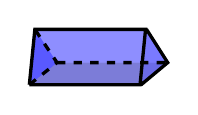
\begin{tikzpicture}[x=2em, y=2em,baseline=0.5em]
    \begin{scope}[very thick]
    \fill[fill=blue, opacity=0.3]
        (0,0)--(2,0)--(2.1,1)--(0.1,1)--(0,0);
    \fill[fill=blue!50!black, opacity=0.3]
        (0,0)--(0.5,0.4)--(2.5,0.4)--(2,0)--(0,0);
    \fill[fill=blue, opacity=0.2]
        (0.1,1)--(0.5,0.4)--(2.5,0.4)--(2.1,1)--(0.1,1);
    \fill[fill=blue, opacity=0.5]
        (0.1,1)--(0.5,0.4)--(0,0)--(0.1,1);
    \fill[fill=blue, opacity=0.4]
        (2,0)--(2.5,0.4)--(2.1,1);
    \draw
        (0,0)--(2,0)--(2.1,1)--(0.1,1)--(0,0)
        (2.02,0)--(2.5,0.4)--(2.117,1.001);
    \draw[dashed]
        (0,0)--(0.5,0.4)--(0.1,1)
        (0.5,0.4)--(2.5,0.4);
    \end{scope}
    \end{tikzpicture}
	\arrow["\bigcup\psi", from=1-1, to=1-3]
	\arrow[from=1-1, to=2-1]
	\arrow[from=2-1, to=3-1]
	\arrow["{\psi_f}"', from=3-1, to=2-3]
	\arrow["\lambda"', dashed, from=2-1, to=1-3]
\end{tikzcd}\]

We reparametrize the relative homotopy into the desired map $\psi_f$ as follows:
\begin{center}
    \begin{tikzcd}
    (\ns\times e_0)\cup(\de\ns\times\sx{1})\times[0,1] \arrow[d] \arrow[r, "H"] & X \\
    \ns\times\sx{1} \arrow[ur, dashed, swap, "\psi_f"]
    \end{tikzcd}
\end{center}\rightnote{He added a nice drawing here illustrating this "reparametrization". The "\'Alvaro pls" Signal /\textbackslash\ means that I would like some picture to be here eventually.}
considering the continuous quotient map.
\begin{center}
    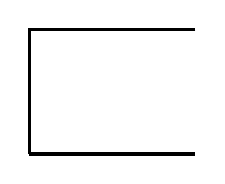
\begin{tikzpicture}[x=6em, y=1.5em,baseline=0.5em]
    \draw[very thick] (0,0)--(1,0) (1,3)--(0,3)--(0,0);
    \end{tikzpicture} \hspace{2em}
    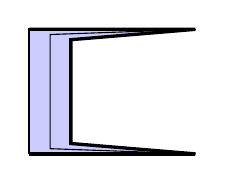
\begin{tikzpicture}[x=6em, y=1.5em,baseline=0.5em]
    \draw[very thick] (0,0)--(1,0) (1,3)--(0,3)--(0,0);
    \def\n{8}
    \def\t{2}
    \def\m{1/\n}
    \foreach \i in {\t,...,0}{
        % the first point is (x, x)
        % the second one is (x, 3-x)
        \filldraw[fill=blue!20] (0,0)--(1,0)--(\i*\m,\i*\m)--(\i*\m, 3-\i*\m)--(1,3)--(0,3);
    }
    \draw[very thick] (0,0)--(1,0)--(\t*\m,\t*\m)--(\t*\m, 3-\t*\m)--(1,3)--(0,3);
    \end{tikzpicture} \hspace{2em}
    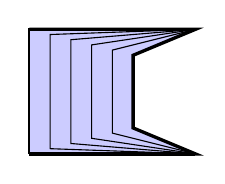
\begin{tikzpicture}[x=6em, y=1.5em,baseline=0.5em]
    \draw[very thick] (0,0)--(1,0) (1,3)--(0,3)--(0,0);
    \def\n{8}
    \def\t{5}
    \def\m{1/\n}
    \foreach \i in {\t,...,0}{
        % the first point is (x, x)
        % the second one is (x, 3-x)
        \filldraw[fill=blue!20] (0,0)--(1,0)--(\i*\m,\i*\m)--(\i*\m, 3-\i*\m)--(1,3)--(0,3);
    }
    \draw[very thick] (0,0)--(1,0)--(\t*\m,\t*\m)--(\t*\m, 3-\t*\m)--(1,3)--(0,3);
    \end{tikzpicture} \hspace{2em}
    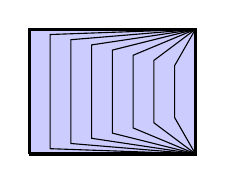
\begin{tikzpicture}[x=6em, y=1.5em,baseline=0.5em]
    \filldraw[very thick, fill=blue!20] (0,0)--(1,0)--(1,3)--(0,3)--(0,0);
    \def\n{8}
    \foreach \i in {0,...,\n}{
        \def\m{1/\n}
        % the first point is (x, x)
        % the second one is (x, 3-x)
        \draw (1,0)--(\i*\m,\i*\m)--(\i*\m, 3-\i*\m)--(1,3);
    }
    \end{tikzpicture}
\end{center}

Now we "adjoin" the continuous maps $\psi_f$ into the simplicial deformation retraction
\[H:S(X)\times\Delta[1]\to S(X)\]

In the simplicial dimension $n$, we need to specify a map
\[S(X)_n\times\Delta([n],[1])\to S(X)_n\]

We do this via an adjunction bijection:
\begin{multline*}
    \Hom_\sSet(Z\times\Delta[1],S(X))\cong\\
    \cong\cb{\psi_f:\nabla^n\times\nabla^1\to X \text{ for all } n\geq0, z\in Z_n,\text{ such that } \psi_{\alpha^*(z)}=\psi_Z(\alpha_*\circ\nabla^1)}
\end{multline*}

\textit{Sketch} (full argument as an exercise).

Step 1. Given $H:Z\times\Delta[1]\to Y$ and $z\in Z_n$, we define $\psi_z:\Delta[n]\times\Delta[1]\to Y$ by $(\psi_z)_m(\alpha,k)=H_m(\alpha^*(z),k)$ (this is bijective by the Yoneda lemma).

Step 2. $\S:\Top\to\sSet$ is right adjoint to $|-|:\sSet\to\Top$ and there is a preferred homeomorphism $|\Delta[n]|\cong\ns$, $(\alpha:[n]\to[m],t)\mapsto\alpha_*(t)$, with inverse $s\mapsto[\id_{[n]},s]$.

Step 3. The map $|\Delta[n]\times\Delta[1]|\xto{(|\pr_1|,|\pr_2|)}|\Delta[n]|\times|\Delta[1]|\cong\ns\times\sx{1}$ is a homeomorphism.

Step 4. Combine steps 1-3.
\begin{align*}
    \Hom_\sSet(Z\times\Delta[1],\S(X))&\underset{\text{Step 1}}{\cong}\cb{\psi_z:\Delta[n]\times\Delta[1]\to\S(X)\mid(\psi_z)_m(\alpha,k)=H_m(\alpha^*(z),k)} \\
    &\underset{\text{Step 2}}{\cong}\cb{\psi_z^\#:|\Delta[n]\times\Delta[1]|\to X} \\
    &\underset{\text{Step 3}}{\cong}\cb{\hat\psi_z:\ns\times\sx{1}\to X}
\end{align*}\todo{I might have written some dumb things}

\end{proof}
